\documentclass[12pt]{article}
\usepackage[a4paper,margin=2.5cm]{geometry}
\usepackage{tikz}
\usepackage{xcolor}
\usetikzlibrary{arrows.meta}
\definecolor{goldenrod}{RGB}{201,162,39}

\begin{document}

\section*{Garis Bilangan Pecahan: Ruas 0 sampai 2 dalam Pertiga}

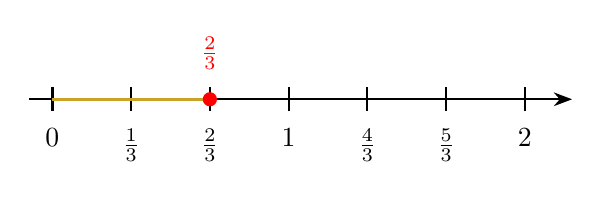
\begin{tikzpicture}[x=1cm]
  % Sumbu dari 0 sampai 2 (6 pertiga)
  \draw[thick,-{Stealth}] (-0.3,0) -- (6.6,0);
  % Tanda untuk setiap pertiga, dari 0 sampai 2
  \foreach \i/\lab in {0/0, 1/\frac{1}{3}, 2/\frac{2}{3},
                        3/1, 4/\frac{4}{3}, 5/\frac{5}{3}, 6/2} {
    \draw[thick] (\i,-0.15) -- (\i,0.15);
    \node[below] at (\i,-0.25) {$\lab$};
  }
  % Ruas 0 sampai 2/3 ditebalkan dengan warna emas
  \draw[very thick, color=goldenrod] (0,0) -- (2,0);
  % Titik pecahan yang sedang dibahas
  \fill[red] (2,0) circle (0.09);
  \node[above, red] at (2,0.25) {$\frac{2}{3}$};
\end{tikzpicture}

\section*{Membandingkan $\frac{2}{3}$ dan $\frac{3}{4}$ pada Dua Garis Sejajar}

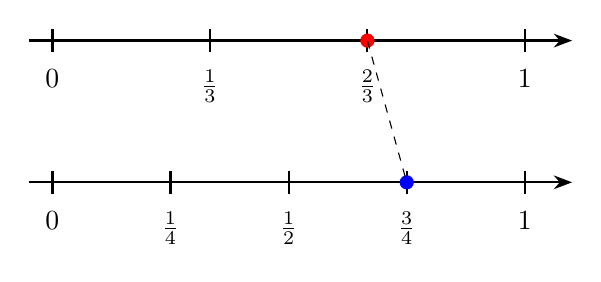
\begin{tikzpicture}[x=1cm]
  % Garis pertiga (atas) dan garis perempat (bawah), sama panjang 6 cm
  \draw[thick,-{Stealth}] (-0.3,0) -- (6.6,0);
  \draw[thick,-{Stealth}] (-0.3,-1.8) -- (6.6,-1.8);
  \foreach \i/\lab in {0/0, 1/\frac{1}{3}, 2/\frac{2}{3}, 3/1} {
    \draw[thick] (2*\i,-0.15) -- (2*\i,0.15);
    \node[below] at (2*\i,-0.25) {$\lab$};
  }
  \foreach \i/\lab in {0/0, 1/\frac{1}{4}, 2/\frac{1}{2}, 3/\frac{3}{4}, 4/1} {
    \draw[thick] (1.5*\i,-1.95) -- (1.5*\i,-1.65);
    \node[below] at (1.5*\i,-2.05) {$\lab$};
  }
  % Titik yang dibandingkan, dihubungkan garis putus-putus
  \fill[red] (4,0) circle (0.09);
  \fill[blue] (4.5,-1.8) circle (0.09);
  \draw[dashed] (4,0) -- (4.5,-1.8);
\end{tikzpicture}

\end{document}
